
\section{A-Fast-RCNN: Approach Details}
We now describe the details of our framework. We first give a brief overview of our base detector Fast-RCNN. This is followed by describing the space of adversarial generation. In particular, we focus on generating different types of occlusions and deformations in this paper. Finally, in Section~\ref{sec:exp}, we describe our experimental setup and show the results which indicate significant improvements over baselines.

\begin{figure*}
    \centering
    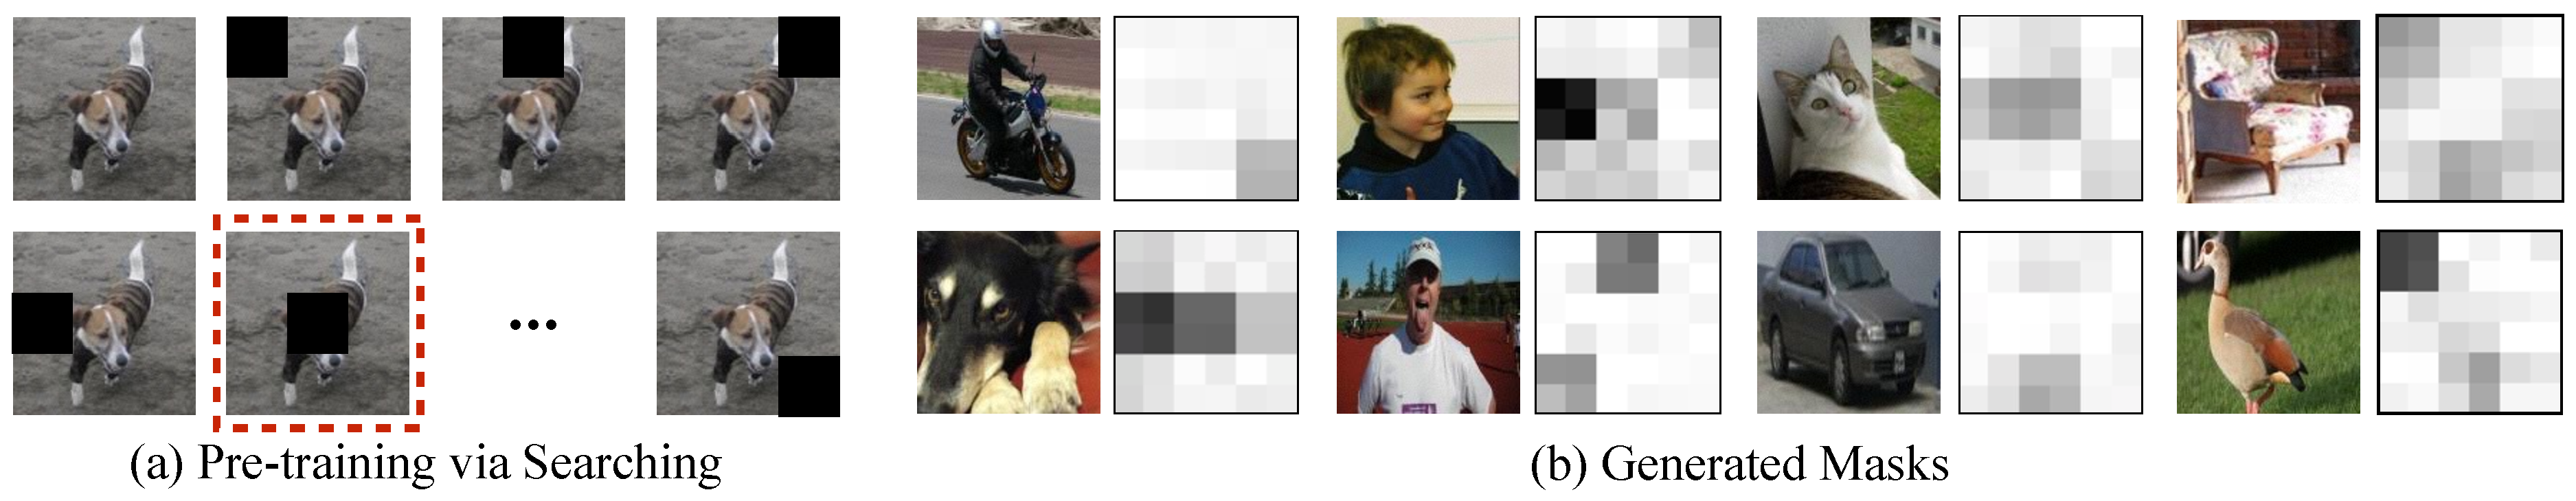
\includegraphics[width=1\textwidth]{masks.pdf}
    \caption{(a) Model pre-training: Examples of occlusions that are sifted to select the hard occlusions and used as ground-truth to train the ASDN network  (b) Examples of occlusion masks generated by ASDN network. The black regions are occluded when passed on to FRCN pipeline. }\label{fig:ASDN}
\end{figure*}

\subsection{Overview of Fast-RCNN}
We build upon the Fast-RCNN framework for object detection~\cite{frcn}. Fast-RCNN is composed of two parts: (i) a convolutional network for feature extraction; (ii) an RoI network with an  RoI-pooling layer and a few fully connected layers that output object classes and bounding boxes. 

Given an input image, the convolutional network of the Fast-RCNN takes the whole image as an input and produces convolutional feature maps as the output. Since the operations are mainly convolutions and max-pooling, the spatial dimensions of the output feature map will change according to the input image size. Given the feature map, the RoI-pooling layer is used to project the object proposals~\cite{Uijlings13} onto the feature space. The RoI-pooling layer crops and resizes to generate a fixed size feature vector for each object proposal. These feature vectors are then passed through fully connected layers. The outputs of the fully connected layers are: (i) probabilities for each object class including the background class; and (ii) bounding box coordinates. 

For training, the SoftMax loss and regression loss are applied on these two outputs respectively, and the gradients are back propagated  though all the layers to perform end-to-end learning.

\subsection{Adversarial Networks Design}
We consider two types of feature generations by adversarial networks competing against the Fast-RCNN (FRCN) detector. The first type of generation is occlusion. Here, we propose Adversarial Spatial Dropout Network (ASDN) which learns how to occlude a given object such that it becomes hard for FRCN to classify. The second type of generation we consider in this paper is deformation. In this case, we propose Adversarial Spatial Transformer Network (ASTN) which learns how to rotate ``parts'' of the objects and make them hard to recognize by the detector. By competing against these networks and overcoming the obstacles, the FRCN learns  to handle object occlusions and deformations in a robust manner. Note that both the proposed networks ASDN and ASTN are learned simultaneously in conjunction with the FRCN during training. Joint training prevents the detector from overfitting to the obstacles created by the fixed policies of generation. 

Instead of creating occlusions and deformations on the input images, we find that operating on the feature space is more efficient and effective. Thus, we design our adversarial networks to modify the features to make the object harder to recognize. Note that these two networks are only applied during training to improve the detector. We will first introduce the ASDN and ASTN individually and then combine them together in an unified framework. 


\subsubsection{Adversarial Spatial Dropout for Occlusion}
We propose an Adversarial Spatial Dropout Network (ASDN) to create occlusions on the deep features for foreground objects. Recall that in the standard Fast-RCNN pipeline, we can obtain the convolutional features for each foreground object proposal after the RoI-pooling layer. We use these region-based features as the inputs for our adversarial network. Given the feature of an object, the ASDN will try to generate a mask indicating which parts of the feature to dropout (assigning zeros) so that the detector cannot recognize the object.

More specifically, given an object we extract the feature $X$ with size $d \times d \times c$, where $d$ is the spatial dimension and  $c$ represents the number of channels (e.g., $c=256, d=6$ in AlexNet). Given this feature, our ASDN will predict a mask $M$ with $d \times d$ values which are either 0 or 1 after thresholding. We visualize some of the masks before thresholding in Fig.~\ref{fig:ASDN}(b). We denote $M_{ij}$ as the value for the $i$th row and $j$th column of the mask. Similarly, $X_{ijk}$ represents the value in channel $k$ at location $i,j$ of the feature. If $M_{ij} = 1$, we drop out the values of all the channels in the corresponding spatial location of the feature map $X$, i.e., $X_{ijk} = 0, \forall k$. 

\textbf{Network Architecture.} We use the standard Fast-RCNN (FRCN) architecture. We initialize the network using pre-training from ImageNet~\cite{imagenet}.  The adversarial network shares the convolutional layers and RoI-pooling layer with FRCN and then uses its own separate fully connected layers. Note that we do not share the parameters in our ASDN with Fast-RCNN since we are optimizing two networks to do the exact opposite tasks. 

\textbf{Model Pre-training.} In our experiment, we find it important to pre-train the ASDN for creating occlusions before using it to improve Fast-RCNN. Motivated by the Faster RCNN detector~\cite{renNIPS15fasterrcnn}, we apply stage-wise training here. We first train our Fast-RCNN detector without ASDN for 10K iterations. As the detector now has a sense of the objects in the dataset, we train the ASDN model for creating the occlusions by fixing all the layers in the detector.

\begin{figure*}[t]
    \centering
    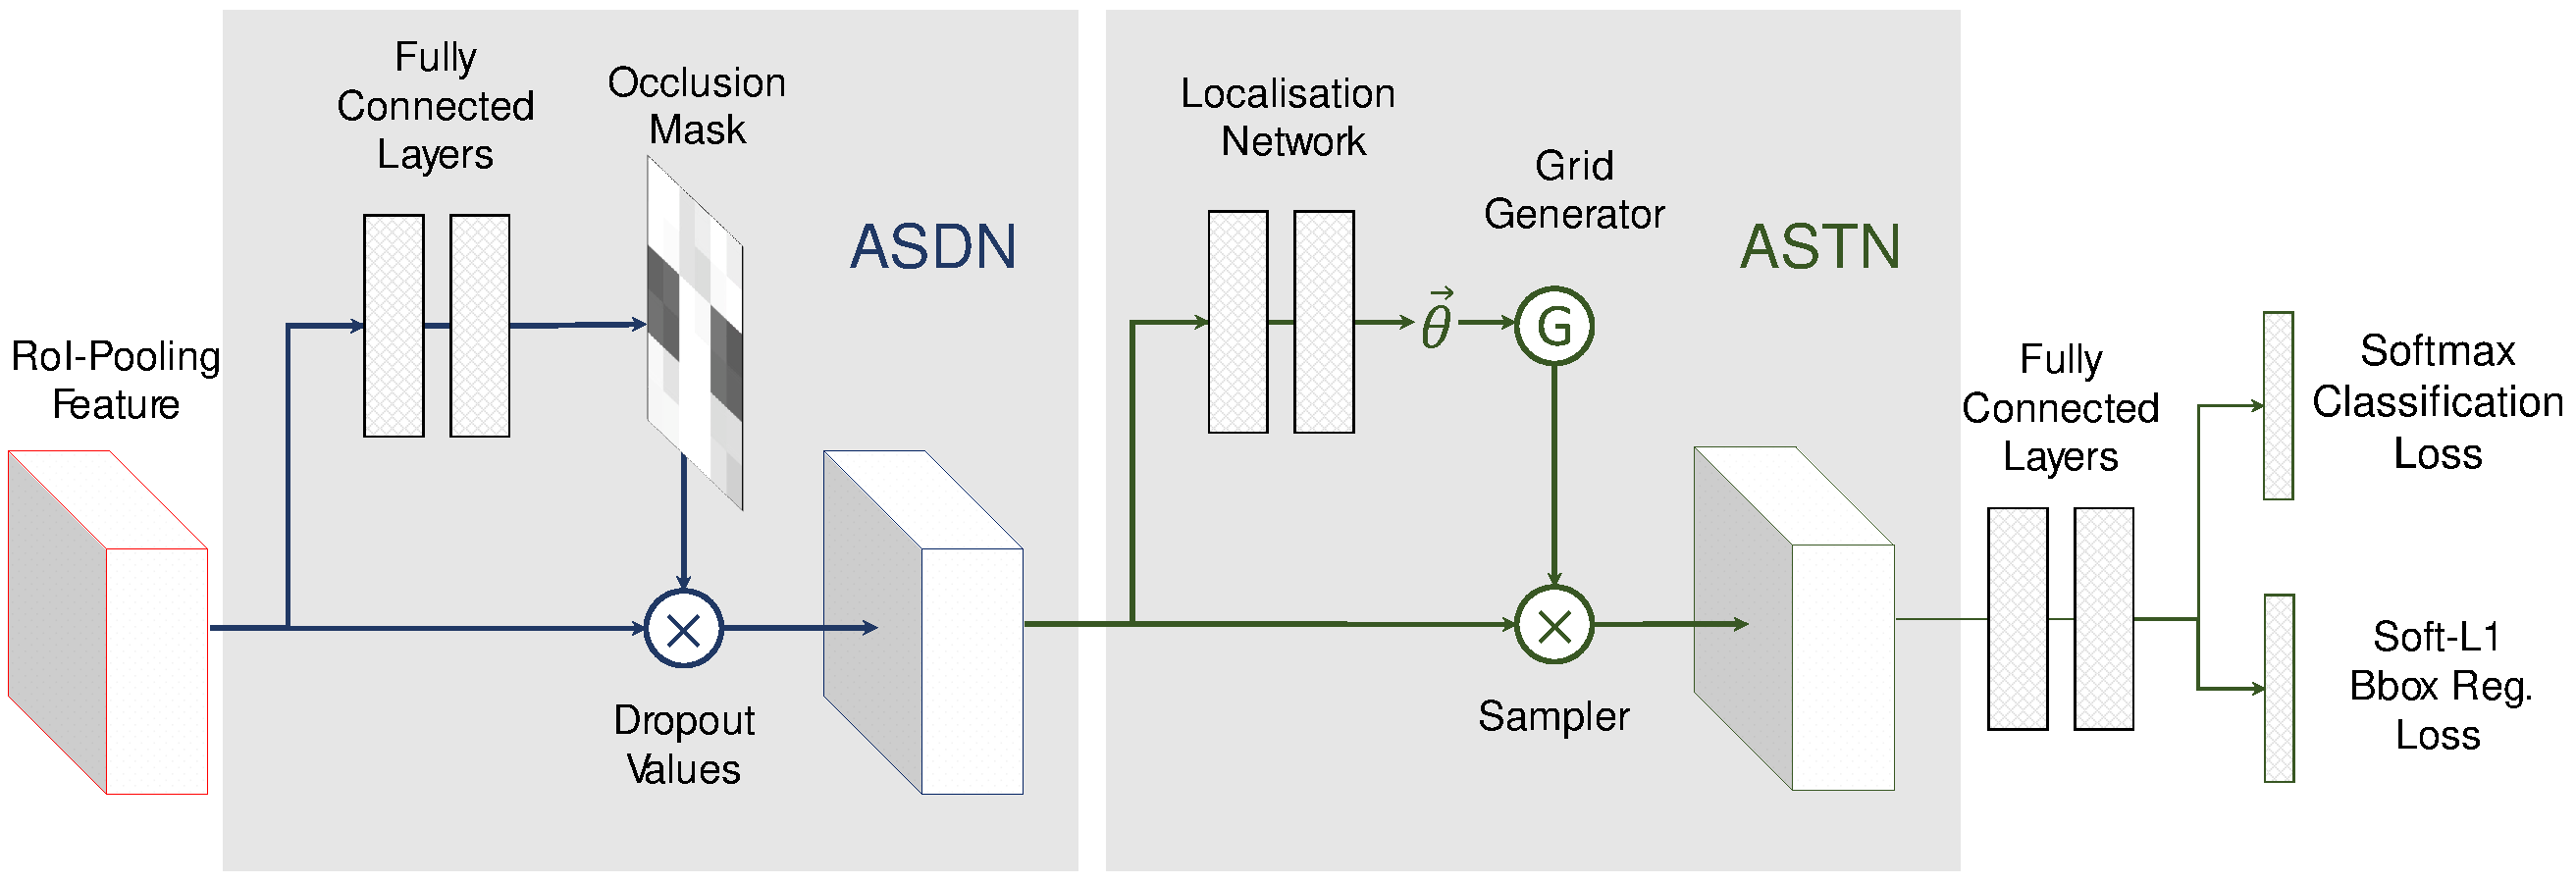
\includegraphics[width=1\textwidth]{network_fusion.pdf}
    \caption{Network architecture for combining ASDN and ASTN network. First occlusion masks are created and then the channels are rotated to generate hard examples for training.}\label{fig:network_fusion}
\end{figure*}

\textbf{Initializing ASDN Network.} To initialize the ASDN network, given a feature map $X$ with spatial layout $d \times d$, we apply a sliding window with size $\frac{d}{3} \times \frac{d}{3}$ on it. We represent the sliding window process by projecting the window back to the image as~\ref{fig:ASDN}(a). For each sliding window, we drop out  the values in all channels whose spatial locations are covered by the window and generate a new feature vector for the region proposal. This feature vector is then passed through classification layers to compute the loss. Based on the loss of all the  $\frac{d}{3} \times \frac{d}{3}$ windows, we select the one with the highest loss. This window is then used to create a single $d \times d$ mask (with 1 for the window location and 0 for the other pixels). We generate these spatial masks for $n$ positive region proposals and obtain $n$ pairs of training examples $\{(X^{1}, \tilde{M}^{1}),..., (X^{n}, \tilde{M}^{n})\}$  for our adversarial dropout network. The idea is that the ASDN should learn to generate the masks which can give the detector network high losses. We apply the binary cross entropy loss in training the ASDN and it can be formulated as,
{\small
\begin{eqnarray}\label{eq:loss_mask}
\mathcal{L} =  - \frac{1}{n} \sum_{p}^{n} \sum_{i, j}^{d} [\tilde{M}_{ij}^p \mathcal{A}_{ij}(X^p) + (1 - \tilde{M}_{ij}^p) (1 - \mathcal{A}_{ij}(X^p)) ], 
\end{eqnarray}
}
where $\mathcal{A}_{ij}(X^p)$ represents the outputs of the ASDN in location $(i,j)$ given input feature map $X^p$. We train the ASDN with this loss for 10K iterations. We show that the network starts to recognize which part of the objects are significant for classification as shown in Fig.~\ref{fig:ASDN}(b). Also note that our output masks are different from the Attention Mask proposed in~\cite{ruslanattention}, where they use the attention mechanism to facilitate classification. In our case, we use the masks to occlude parts to make the classification harder. 




\textbf{Thresholding by Sampling.} The output generated by ASDN network is not a binary mask but rather a continuous heatmap. Instead of using direct  thresholding, we use importance sampling to select the top $\frac{1}{3}$ pixels to mask out. Note that the sampling procedure incorporates stochasticity and diversity in samples during training. More specifically, given a heatmap, we first select the top $\frac{1}{2}$ pixels with top probabilities and randomly select $\frac{1}{3}$ pixels out of them to assign the value 1 and the rest of $\frac{2}{3}$ pixels are set to 0. 





\textbf{Joint Learning.}  Given the pre-trained ASDN and Fast-RCNN model, we jointly optimize these two networks in each iteration of training. For training the Fast-RCNN detector, we first use the ASDN to generate the masks on the features after the RoI-pooling during forward propagation. We perform sampling to generate binary masks and use them to drop out the values in the features after the RoI-pooling layer. We then forward the modified features to calculate the loss and train the detector end-to-end. Note that although our features are modified, the labels remain the same. In this way, we create ``harder'' and more diverse examples for training the detector. 

For training the ASDN, since we apply the sampling strategy to convert the heatmap into a binary mask, which is not differentiable, we cannot directly back-prop the gradients from the classification loss. Alternatively, we take the inspirations  from the REINFORCE~\cite{reinforce} approach. We compute  which binary masks lead to significant drops in Fast-RCNN classification scores. We use only those hard example masks as ground-truth to train the adversarial network directly using the same loss as described in Eq.~\ref{eq:loss_mask}.




\vspace{-0.05in}
\subsubsection{Adversarial Spatial Transformer Network}
\vspace{-0.05in}
We now introduce the Adversarial Spatial Transformer Network (ASTN). The key idea is to create deformations on the object features and make object recognition by the detector difficult. Our network is built upon the Spatial Transformer Network (STN) proposed in~\cite{stn15}. In their work, the STN is proposed to deform the features to make classification easier. Our network, on the other hand, is doing the exact opposite task. By competing against our ASTN, we can train a better detector which is robust to deformations. 

\textbf{STN Overview.} The Spatial Transformer Network~\cite{stn15} has three components: localisation network, grid generator and sampler. Given the feature map as input, the localisation network will estimate the variables for deformations (e.g., rotation degree, translation distance and scaling factor). These variables will be used as inputs for the grid generator and sampler to operate on the feature map. The output is a deformed feature map. Note that we only need to learn the parameters in the localisation network. One of the key contribution of STN is making the whole process differentiable, so that the localisation network can be directly optimized for the classification objective via back propagation. Please refer to~\cite{stn15} for more technical details. 



\textbf{Adversarial STN.} In our Adversarial Spatial Transformer Network, we focus on feature map rotations. That is, given a feature map after the RoI-pooling layer as input, our ASTN will learn to rotate the feature map to make it harder to recognize. Our localisation network is composed with 3 fully connected layers where the first two layers are initialized with fc6 and fc7 layers from ImageNet pre-trained network as in our Adversarial Spatial Dropout Network. 

We train the ASTN and the Fast-RCNN detector jointly. For training the detector, similar to the process in the ASDN, the features after RoI-pooling are first transformed by our ASTN and forwarded to the higher layers to compute the SoftMax loss. For training the ASTN, we optimize it so that the detector will classify the foreground objects as the background class. Different from training ASDN, since the spatial transformation is differentiable, we can directly use the classification loss to back-prop and finetune the parameters in the localisation network of ASTN. 

\textbf{Implementation Details.} In our experiments, we find it very important to limit the rotation degrees produced by the ASTN. Otherwise it is very easy to rotate the object upside down which is the hardest to recognize in most cases. We constrain the rotation degree within  10{\degree} clockwise and anti-clockwise. Instead of rotating all the feature map in the same direction, we divide the feature maps on the channel dimension into 4 blocks and estimate 4 different rotation angles for different blocks. Since each of the channel corresponds to activations of one type of feature, rotating channels separately corresponds to rotating parts of the object in different directions which leads to deformations. We also find that if we use one rotation angle for all feature maps, the ASTN will often predict the largest angle. By using 4 different angles instead of one, we increase the complexity of the task which prevents the network from predicting trivial deformations. 

\vspace{-0.1in}
\subsubsection{Adversarial Fusion}
\vspace{-0.05in}
The two adversarial networks ASDN and ASTN can also be combined and trained together in the same detection framework. Since these two networks offer different types of information. By competing against these two networks simultaneously, our detector become more robust. 

We combine these two networks into the Fast-RCNN framework in a sequential manner. As shown in Fig.~\ref{fig:network_fusion}, the feature maps extracted after the RoI-pooling are first forwarded to our ASDN which drop out some activations. The modified features are further deformed by the ASTN. 








